% Results
% -----------------------------
\section{Results}

\begin{frame}
  \sectionpage
\end{frame}

\begin{frame}{Handling heterogeneity}
  \begin{columns}
    \begin{column}{.4\textwidth}
      \begin{figure}
              \captionsetup{justification=centering}
        \includegraphics<1>[width=\linewidth,left]{./figures/eval/clustering/clustering_benign.pdf}%
        \caption{Clustering results without poisoning.\\ 
        Rand index=1.0}
      \end{figure}
    \end{column}
  \begin{column}{.6\textwidth}

\begin{table}
    \centering
    \caption*{Accuracy for different baselines.}
    \footnotesize
    \setlength\tabcolsep{1ex}
    \begin{tabularx}{.7\textwidth}{X|ccc}
      \toprule % ---------------------------------
      \textbf{Scenario}
      & \multicolumn{1}{c}{\texttt{RADAR}} & \multicolumn{1}{c}{\texttt{FoolsGold}} & \multicolumn{1}{c}{\texttt{Clustered}} \\
      \midrule % ---------------------------------
      \textbf{Benign} & \hg 99.07 & \hr 55.04 & \hg 99.24  \\
    \end{tabularx}
    \caption*{\smaller More is better}

  \end{table}
    \end{column}
  \end{columns}
\end{frame}

%%%%%%%%%%%%
%Untargeted
%%%%%%%%%%%%
\begin{frame}{Handling Untargeted Attacks}
  \begin{columns}
    \begin{column}{.4\textwidth}
      \begin{figure}
        \captionsetup{justification=centering}
        \only<1>{
            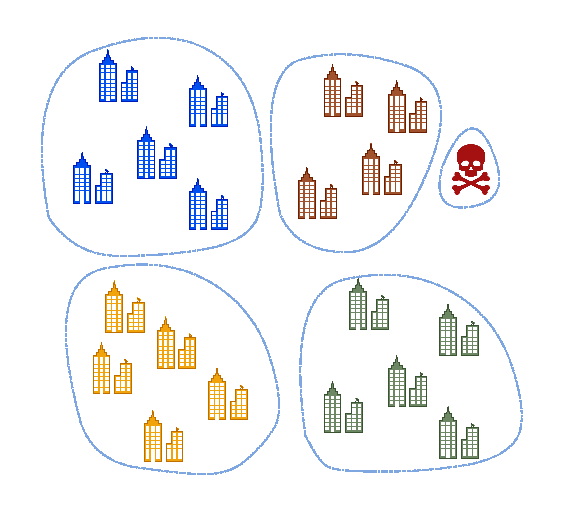
\includegraphics[width=\linewidth,left]{./figures/eval/clustering/clustering_lone_untargeted.pdf}
            \caption*{Clustering results for\\
            \texttt{lone 100U}.\\ 
            Rand index=1.0
            }
        }
        \only<2>{
            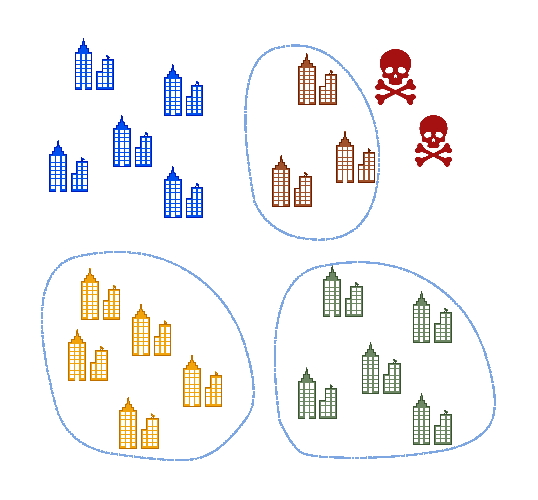
\includegraphics[width=\linewidth,left]{./figures/eval/clustering/clustering_min_untargeted.pdf}
            \caption*{Clustering results for\\ \texttt{colluding minority 100U}\\ 
            Rand index=1.0
            }
        }
        \only<3>{
            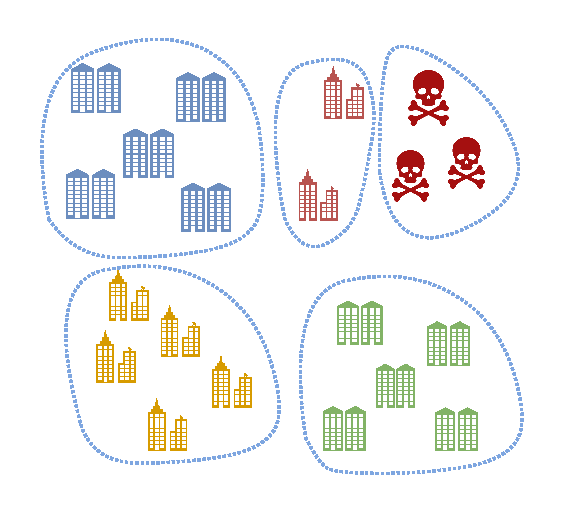
\includegraphics[width=\linewidth,left]{./figures/eval/clustering/clustering_maj_untargeted.pdf}
          \caption*{Clustering results for\\
            \texttt{colluding majority 100U}\\ 
            Rand index=1.0
            }
        }        
      \end{figure}
    \end{column}

  \begin{column}{.6\textwidth}
    \begin{table}
        \centering
    
        \footnotesize
        \setlength\tabcolsep{1ex}
        \caption*{Attack success rate for different baselines.}  
        \begin{tabularx}{.8\textwidth}{lXccc}
          \toprule % ---------------------------------
          \multicolumn{2}{c}{{\textbf{Scenario}}}
          & \multicolumn{1}{c}{\texttt{RADAR}} & \multicolumn{1}{c}{\texttt{FoolsGold}} & \multicolumn{1}{c}{\texttt{Clustered}} \\
          \midrule % ---------------------------------
          % % UNTARGETED ATTACKS
          \multicolumn{2}{l}{\textbf{Untargeted} (\texttt{100U})}  & & & \\
          & \texttt{Lone} & \hg 0.08 &\hr 99.89 & \hg 0.12 \\
          \only<2->{& \texttt{Collud. min.} & \hg 0.10 & \hg 0.04 &\ho 6.26 \\}
          \only<3->{& \texttt{Collud. maj.} & \hg 0.08 &\ho 38.98 & \hr 94.36 \\}
          \end{tabularx}
          \caption*{\smaller Less is better}
      \end{table}
  
     \end{column}
  \end{columns}
\end{frame}


%%%%%%%%%%%%    
% Targeted   
%%%%%%%%%%%%

\begin{frame}{Handling Targeted Attacks}
    \begin{columns}
        \begin{column}{.4\textwidth}
            \begin{figure}
                \centering
                \captionsetup{justification=centering}
                \only<1-2>{%
                    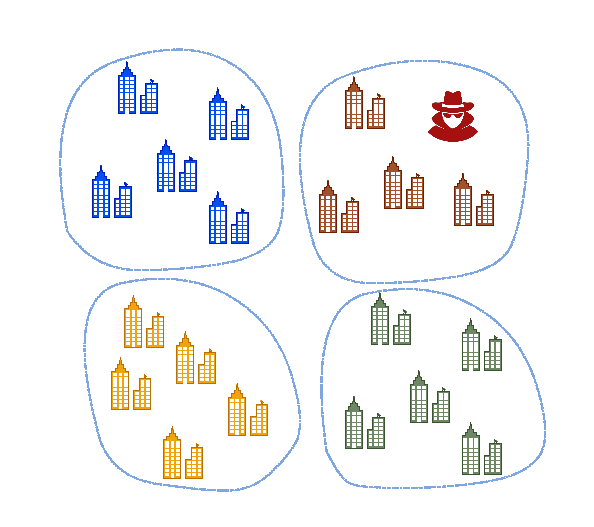
\includegraphics[width=\linewidth,left]{figures/eval/clustering/clustering_lone_targeted.pdf}
                    \caption*{
                        Clustering results for\\
                        \texttt{Lone 100T}\\ 
                        Rand index=0.97
                    }
                }
                \only<3>{%
                    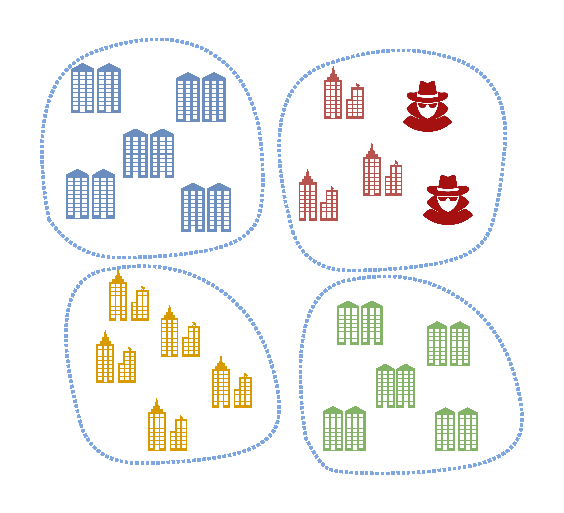
\includegraphics[width=\linewidth,left]{./figures/eval/clustering/clustering_min_targeted.pdf}%
                    \caption*{
                        Clustering results for\\
                        \texttt{colluding minority 100T}\\ 
                        Rand index=0.97
                    }
                }
                \only<4-5>{
                    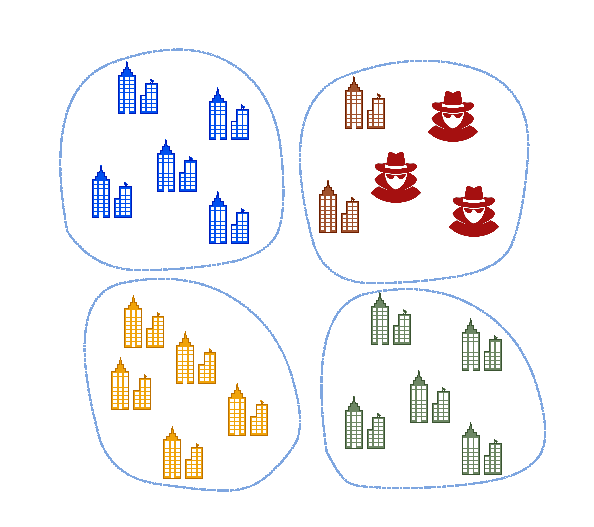
\includegraphics[width=\linewidth,left]{./figures/eval/clustering/clustering_maj_targeted.pdf}%
                    \caption*{Clustering results for \texttt{colluding majority 100T}\\ 
                    Rand index=0.96}
                }
                
            \end{figure}
        \end{column}
        \begin{column}{.6\textwidth}
            \begin{table}
                \centering
                \footnotesize
                \setlength\tabcolsep{1ex}
                \caption*{Attack success rate for different baselines.}  

                \begin{tabularx}{.8\textwidth}{lXccc}
                    \toprule % ---------------------------------
                    \multicolumn{2}{c}{{\textbf{Scenario}}}
                    & \multicolumn{1}{c}{\texttt{RADAR}} & \multicolumn{1}{c}{\texttt{FoolsGold}} & \multicolumn{1}{c}{\texttt{Clustered}} \\
                    \midrule % ---------------------------------
                    % % TARGETED ATTACKS
                    \multicolumn{2}{l}{\textbf{Targeted} (\texttt{100T})}  & & & \\    
                    & \texttt{Lone} &\hg 0.00 & \hr 93.82 & \hg 0.45 \\
                    \only<3->{& \texttt{Collud. min.} & \hg 0.00 & \hg 2.97 & \hr 53.40 \\}
                    \only<4->{& \texttt{Collud. maj.} &  \hr 73.39 & \ho 8.10 & \hr 59.36 \\}
                \end{tabularx}
                
                \caption*{\smaller Less is better}
            \end{table}
            \vspace{-1em}
            
            \only<2>{\begin{minipage}{\textwidth}
                \begin{figure}
                    \captionsetup{justification=centering}
                    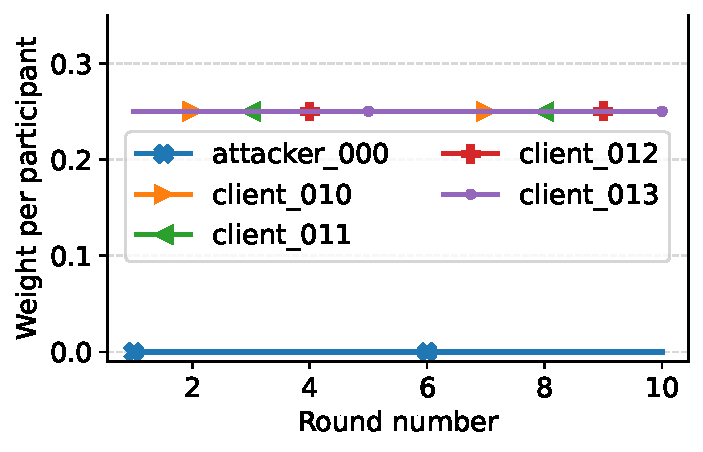
\includegraphics[width=.6\linewidth]{./figures/eval/reput/lone_loud_expanded.pdf}
                    \caption{Aggregation weights.}
                \end{figure}
            \end{minipage}}

            \only<5>{\begin{minipage}{\textwidth}
                \begin{figure}
                    \captionsetup{justification=centering}
                    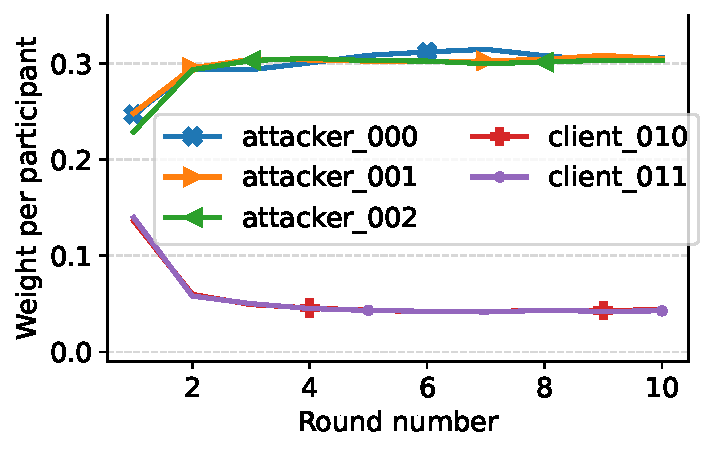
\includegraphics[width=.6\linewidth]{./figures/eval/reput/byzantine_majority_loud_expanded.pdf}
                    \caption{Aggregation weights.}
                \end{figure}
           \end{minipage}}

        \end{column}
    \end{columns}
\end{frame}


% \begin{frame}{Handling targeted attacks}
%   \begin{columns}
%     \begin{column}{.4\textwidth}
    
%       \begin{tikzpicture}
%         \node[] (t1) at (0, 0) {
%           \includegraphics<1>[width=\linewidth]{./figures/eval/clustering/clustering_lone_targeted.pdf}
%         };
%       \end{tikzpicture}
%       \vspace{-0.5cm}
%       \begin{figure}
      
%         \captionsetup{justification=centering}
%         \caption*{Clustering results for\\
%         \texttt{Lone 100T}\\ 
%         Rand index=0.97}
%       \end{figure}

%     \end{column}    
%   \begin{column}{.6\textwidth}
%                 \begin{table}
%                     \centering
%                     \footnotesize
%                     \setlength\tabcolsep{1ex}
%                         \caption*{Attack success rate for different baselines.}  
    
%                         \begin{tabularx}{.8\textwidth}{lXccc}
%                             \toprule % ---------------------------------
%                             \multicolumn{2}{c}{{\textbf{Scenario}}}
%                             & \multicolumn{1}{c}{\texttt{RADAR}} & \multicolumn{1}{c}{\texttt{FoolsGold}} & \multicolumn{1}{c}{\texttt{Clustered}} \\
%                             \midrule % ---------------------------------
%                             % % TARGETED ATTACKS
%                             \multicolumn{2}{l}{\textbf{Targeted} (\texttt{100T})}  & & & \\    
%                             & \texttt{Lone} &\hg \tikz[baseline]{ \node[anchor=base] (t2){0.00}}  & \hr 93.82 & \hg 0.45 \\
%                         \end{tabularx}  
%                 \caption*{\smaller Less is better}

%                 \end{table}
%                 \vspace{0.5cm}
%                 % \begin{columns}
%                 %     \begin{column}{.25\textwidth}
%                 %         \begin{text}{}{
%                 %             \tikz[]{ \node (n1) {Attacker is grouped with \\
%                 %             benign participants ...};} 
%                 %         }
%                 %         \end{text}
%                 %     \end{column}
 
%                 %     \begin{column}{.25\textwidth}
%                 %         \begin{text}{}{\raggedright
%                 %             \tikz[]{ \node (n2) {still, the results are good, why ?};} 
%                 %         }
%                 %         \end{text}
%                 %     \end{column}
%                 % \end{columns}

%                 %     \begin{tikzpicture}[overlay]
%                 %         \path[->]<1-> (n1.north west) edge [bend right] ($(t1.east) + (-0.75,1.75)$);
%                 %     \end{tikzpicture}        
%                 %     \begin{tikzpicture}[overlay]
%                 %         \path[->]<1-> (n2.north east) edge [bend right] (t2);
%                 %     \end{tikzpicture}
%          \end{column}
%   \end{columns}
% \end{frame}

% %%%%%%%%%%%%    
% % Lone bis 
% %%%%%%%%%%%%
% \begin{frame}{Handling targeted attacks: reputation effect}
%   \begin{columns}
%     \begin{column}{.4\textwidth}
%       \begin{figure}
%         \captionsetup{justification=centering}
%         \includegraphics<1>[width=\linewidth,left]{./figures/eval/clustering/clustering_lone_targeted.pdf}%
%         \caption*{Clustering results for\\
%         \texttt{Lone 100T}\\ 
%         Rand index=0.97}
%       \end{figure}
%     \end{column}
%   \begin{column}{.6\textwidth}

%   \begin{minipage}[t][0.35\textheight]{\textwidth}
%             \centering
%             \begin{table}
%                 \centering
%                 \footnotesize
%                 \setlength\tabcolsep{1ex}
%                 \caption*{Attack success rate for different baselines.}
%                     \begin{tabularx}{.8\textwidth}{lXccc}
%                         \toprule % ---------------------------------
%                         \multicolumn{2}{c}{{\textbf{Scenario}}}
%                         & \multicolumn{1}{c}{\texttt{RADAR}} & \multicolumn{1}{c}{\texttt{FoolsGold}} & \multicolumn{1}{c}{\texttt{Clustered}} \\
%                         \midrule % ---------------------------------
%                         % \multicolumn{2}{l|}{\textbf{Benign}}& \hg 0.00 & \ho 5.17 & \hg 0.09  \\
%                         % % TARGETED ATTACKS
%                         \multicolumn{2}{l}{\textbf{Targeted} (\texttt{100T})}  & & & \\    
%                         & \texttt{Lone} &\hg 0.00  & \hr 93.82 & \hg 0.45 \\
%                     \end{tabularx}
%             \end{table}
%     \end{minipage}
%     \begin{minipage}[t][0.65\textheight]{\textwidth}
%         \begin{figure}
%             \captionsetup{justification=centering}
%                 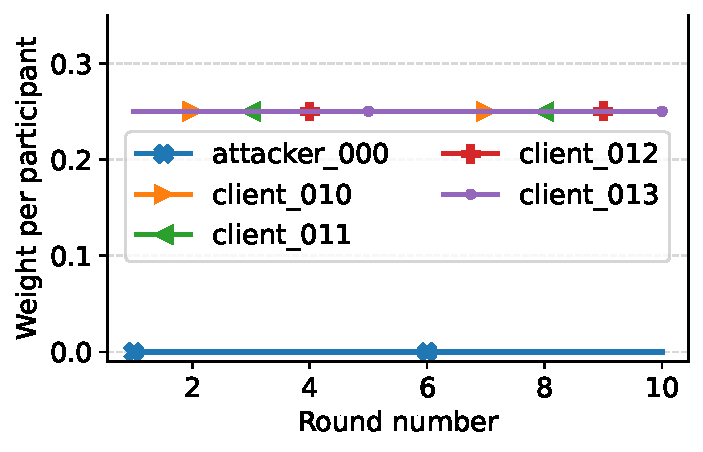
\includegraphics[width=0.65\linewidth]{./figures/eval/reput/lone_loud_expanded.pdf}
%                 \caption{Participants reputation for\\
%                 \texttt{Lone 100T}}
%       \end{figure}
%     \end{minipage}  
  
%     \end{column}
%   \end{columns}
% \addtocounter{framenumber}{-1}
% \end{frame}


% %%%%%%%%%%%%    
% % Targeted min   
% %%%%%%%%%%%%
% \begin{frame}{Handling targeted attacks}
%   \begin{columns}
%     \begin{column}{.4\textwidth}
%       \begin{figure}
%         \captionsetup{justification=centering}
%         \includegraphics<1>[width=\linewidth,left]{./figures/eval/clustering/clustering_min_targeted.pdf}%
%         \caption*{Clustering results for\\
%         \texttt{colluding minority 100T}\\ 
%         Rand index=0.97}
%       \end{figure}
%     \end{column}
%   \begin{column}{.6\textwidth}
%   \begin{minipage}[t][0.35\textheight]{\textwidth}
%                 \centering
%                 \begin{table}
%                     \centering
%                     \footnotesize
%                     \setlength\tabcolsep{1ex}
%                     \caption*{Attack success rate for different baselines.}
%                         \begin{tabularx}{.8\textwidth}{lXccc}
%                             \toprule % ---------------------------------
%                             \multicolumn{2}{c}{{\textbf{Scenario}}}
%                             & \multicolumn{1}{c}{\texttt{RADAR}} & \multicolumn{1}{c}{\texttt{FoolsGold}} & \multicolumn{1}{c}{\texttt{Clustered}} \\
%                             \midrule % ---------------------------------
%                             % \multicolumn{2}{l|}{\textbf{Benign}}& \hg 0.00 & \ho 5.17 & \hg 0.09  \\
%                             % % TARGETED ATTACKS
%                             \multicolumn{2}{l}{\textbf{Targeted} (\texttt{100T})}  & & & \\    
%                             & \texttt{Lone} &\hg 0.00  & \hr 93.82 & \hg 0.45 \\
%                             & \texttt{Collud. min.} & \hg 0.00 & \hg 2.97 & \hr 53.40 \\
%                         \end{tabularx}  
%                         \caption*{\smaller Less is better}
%                 \end{table}
%         \end{minipage}
%         % \vspace{0.25cm}            
%     % \begin{minipage}[t][0.65\textheight]{\textwidth}
%     %     \begin{figure}
%     %     % Matérialiser le zoom du cluster rouge vers les courbes de droites ?  
%     %         \captionsetup{justification=centering}
%     %             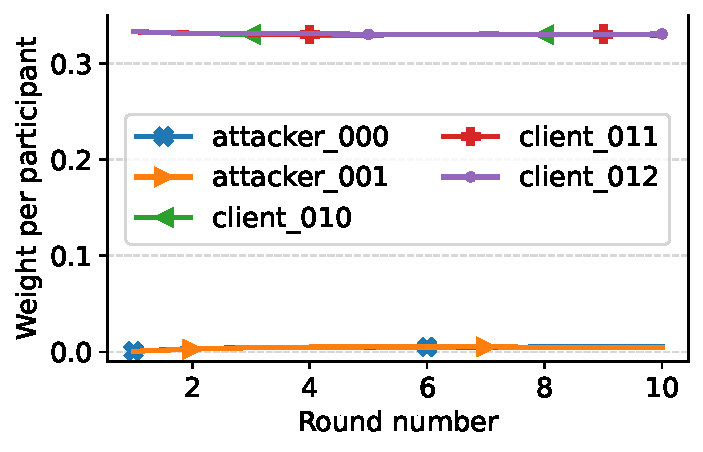
\includegraphics[width=0.65\linewidth]{./figures/eval/reput/byzantine_minority_loud_expanded.pdf}
%     %             \caption{Participants reputation for\\
%     %             \texttt{colluding minority 100T}}
%     %   \end{figure}
%     % \end{minipage}  
%          \end{column}
%   \end{columns}
% \addtocounter{framenumber}{-1}
% \end{frame}

% %%%%%%%%%%%%    
% % Targeted maj   
% %%%%%%%%%%%%
% %Disours
% %Insister sur le fait que c'est un cas hardcore dans lequel les systèmes de réput et de clustering se vautre et que donc nous aussi.
% %A dire dans cet ordre là et pas l'inverse. 
% \begin{frame}{Handling targeted attacks}
%   \begin{columns}
%     \begin{column}{.4\textwidth}
%       \begin{figure}
%         \captionsetup{justification=centering}
%         \includegraphics<1>[width=\linewidth,left]{./figures/eval/clustering/clustering_maj_targeted.pdf}%
%         \caption*{Clustering results for \texttt{colluding majority 100T}\\ 
%         Rand index=0.96}
%       \end{figure}
%     \end{column}
%   \begin{column}{.6\textwidth}

%   \begin{minipage}[t][0.35\textheight]{\textwidth}
%                 \centering
%                 \begin{table}
%                     \centering
%                     \footnotesize
%                     \setlength\tabcolsep{1ex}
%                         \begin{tabularx}{.8\textwidth}{lXccc}
%                             \toprule % ---------------------------------
%                             \multicolumn{2}{c}{{\textbf{Scenario}}}
%                             & \multicolumn{1}{c}{\texttt{RADAR}} & \multicolumn{1}{c}{\texttt{FoolsGold}} & \multicolumn{1}{c}{\texttt{Clustered}} \\
%                             \midrule % ---------------------------------
%                             % % TARGETED ATTACKS
%                             \multicolumn{2}{l}{\textbf{Targeted} (\texttt{100T})}  & & & \\    
%                             & \texttt{Lone} &\hg 0.00  & \hr 93.82 & \hg 0.45 \\
%                             & \texttt{Collud. min.} & \hg 0.00 & \hg 2.97 & \hr 53.40 \\
%                             & \texttt{Collud. maj.} &  \hr 73.39 & \ho 8.10 & \hr 59.36 \\
%                         \end{tabularx}  
%                 \end{table}
%         \end{minipage}
%     \begin{minipage}[t][0.65\textheight]{\textwidth}
%         \begin{figure}
%             \captionsetup{justification=centering}
%                 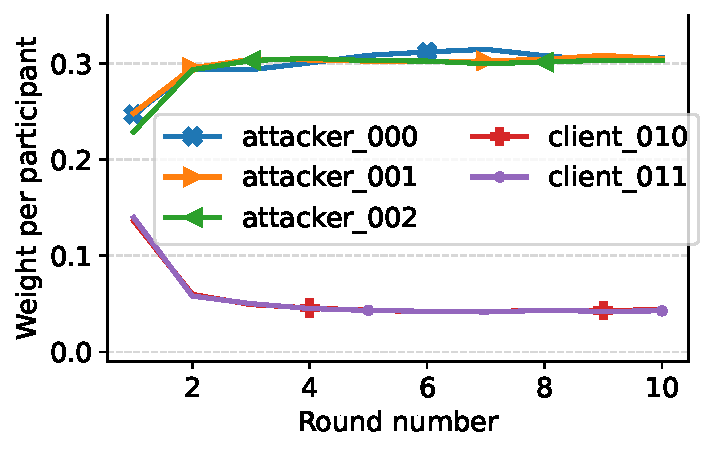
\includegraphics[width=0.65\linewidth]{./figures/eval/reput/byzantine_majority_loud_expanded.pdf}
%                 \caption*{Participants reputation for\\
%                 \texttt{colluding majority 100T}}
%       \end{figure}
%     \end{minipage}  
%          \end{column}
%   \end{columns}
% \addtocounter{framenumber}{-1}
% \end{frame}